%%%%%%%%%%%%%%%%%%%%%%%%%%%%%%%%%%%%%
%% Supporting Information
%% (Optional)
%%%%%%%%%%%%%%%%%%%%%%%%%%%%%%%%%%%%%
% OVERVIEW
%
% Please note that all supporting information will be peer reviewed with your manuscript.
% In general, the purpose of the supporting information is to enable
% authors to provide and archive auxiliary information such as data
% tables, method information, figures, video, or computer software,
% in digital formats so that other scientists can use it.

% The key criteria are that the data:
% 1. supplement the main scientific conclusions of the paper but are not essential to the conclusions (with the exception of
%    including data so the experiment can be reproducible);
% 2. are likely to be usable or used by other scientists working in the field;
% 3. are described with sufficient precision that other scientists can understand them, and
% 4. are not exe files.
%

% All Supporting text and figures should be included in this document.

% Data sets, large tables, movie files,
% and audio files should be uploaded separately, following AGU naming
% conventions. Include their captions in this document and list the
% file name with the caption. You will be prompted to upload these
% files on the Upload Files tab during the submission process, using
% file type “Supporting Information (SI)”

%\documentclass{agujournal2018}

% Please type in the journal name: \journalname{<Journal Name>}
% ie,
%\journalname{Geophysical Research Letters}

%% Choose from this list of Journals:
%
% Journal of Geophysical Research
% JGR-Biogeosciences
% JGR-Earth Surface
% JGR-Planets
% JGR-Solid Earth
% JGR-Space Physics
% Global Biochemical Cycles
% Geophysical Research Letters
% Paleoceanography
% Radio Science
% Reviews of Geophysics
% Tectonics
% Space Weather
% Water Resource Research
% Geochemistry, Geophysics, Geosystems
% Journal of Advances in Modeling Earth Systems (JAMES)
% Earth's Future
% Earth and Space Science

\documentclass[main.tex]{subfiles}

\begin{document}

%% This command needs article title as argument to \supportinginfo{}:
%\supportinginfo{Antigorite Creep at Subduction Conditions: Long Duration, High Accuracy Rheological Tests On Intact Cores Using a Re-Designed Griggs Assembly}

%\authors{Eric Burdette and Greg Hirth}


%\affiliation{1}{Department of Earth, Environmental and Planetary Sciences, Brown University, Providence, RI, USA}

%% Corresponding Author
%(include name and email addresses of the corresponding author.  More
%than one corresponding author is allowed in this Word file and for
%publication; but only one corresponding author is allowed in our
%editorial system.)  

%\correspondingauthor{Eric Burdette}{eric\_burdette@brown.edu}

%% ------------------------------------------------------------------------ %%
%
%  TEXT
%
%% ------------------------------------------------------------------------ %%

\section{Supporting Information}

% \section*{Contents}
% %%%Remove or add items as needed%%%
% \begin{enumerate}
% \item Text S1 to Sx
% \item Figures S1 to Sx
% \item Tables S1 to Sx
% \end{enumerate}

% \section*{Additional Supporting Information (Files uploaded separately)}

% \begin{enumerate}
% \item placeholder
% \end{enumerate}

% \section*{Introduction}
%     Here we have included supporting details describing calibration, extensive comparison of our to other work, and detailed methods used to collect and process strain rate data. In addition we have included collected hardening data that illustrates the magnitude of potential uncertainty on the  produced flow law.
% %Delete all unused file types below. 
% %Copy/paste for multiples of each file type as needed.





\subsection{Mechanical Data Calculations} \label{CH2s_mechcalcs}
    The Griggs apparatus has both external load and displacement sensors which need to be corrected to find load and displacement on the sample inside the pressure vessel. Differential stress is determined by subtracting a "hit point" stress (hydrostatic pressure+friction) from the externally measured load. Displacement is determined by subtracting displacement absorbed by the column in compression \citep{burdette2020enhanced}, and referenced relative to the "hit point".
    \begin{equation}
        x_{sample} = x_{LVDT2} - \frac{\sigma_{1, external}}{k_{lower/_column}}
    \end{equation}
    To calculate permanent/inelastic strain, elastic compression of the sample can also be removed:   
    \begin{equation}
        k_{sample} = \frac{E}{l_{sample}}
    \end{equation}
    \begin{equation}
        x_{inelastic} = x_{LVDT2} - \frac{\sigma_{1, external}}{k_{lower\_column}} - \frac{\sigma_{differential, internal}}{k_{sample}}
    \end{equation}
    
    Note that these equations assume sample elasticity is constant, and don't account for rate-dependent friction.
    
    To calculate strain rates during post-processing, we used the first derivative of a first order Savitzky-Golay filter (moving line fit) over a moving time window chosen for each step. For strain rates above $10^{-6} 1/s$, the window could be as short as 100 seconds, while the lowest strain rates require a 10000 second time window. Strain rates chosen for flow law fits were the final point that was not influenced by a disturbance or loading to the next stress. Wherever strain rate is plotted as a continuous function of time (e.g. figure \ref{fig:CH2s_Load-Displacement}), a single window length was chosen over the whole plot to best display data. 

\begin{figure}
  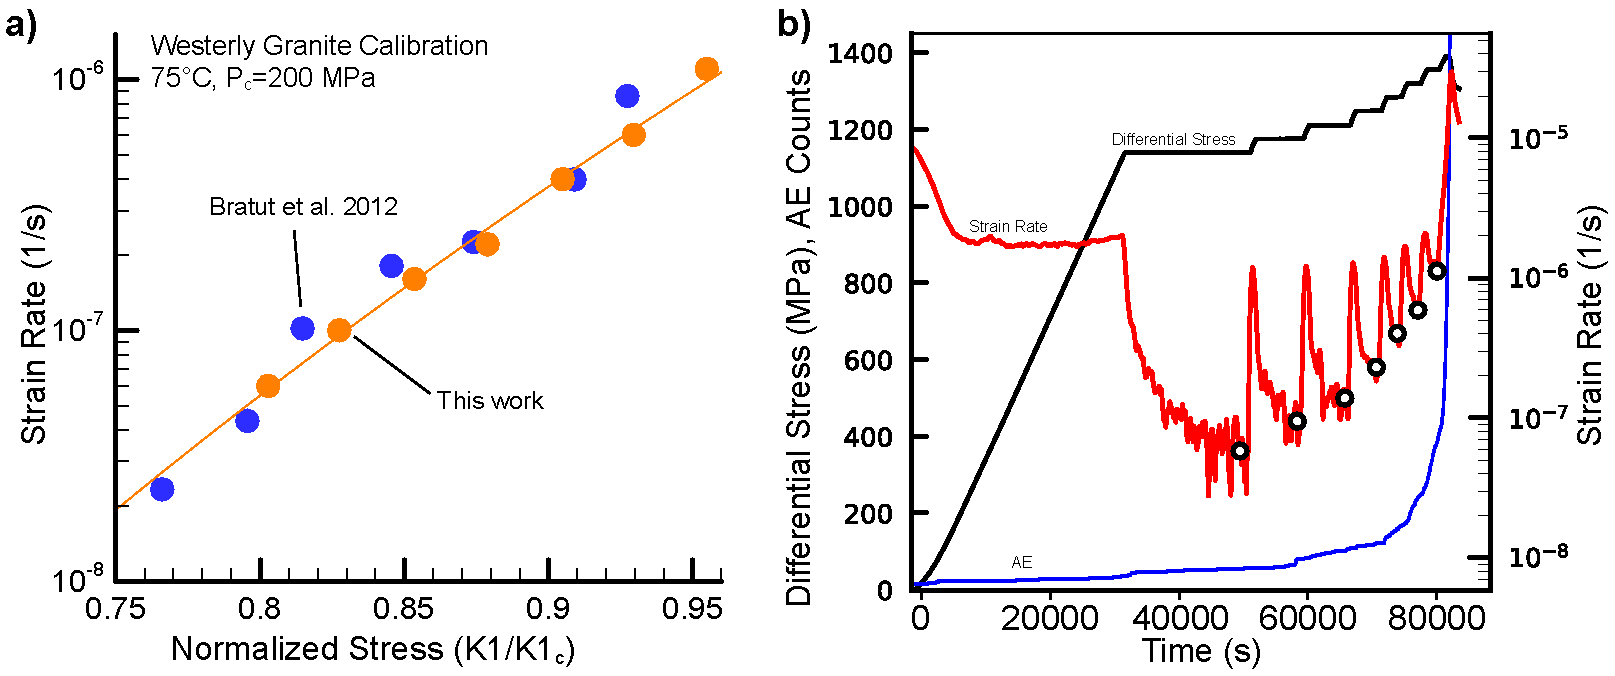
\includegraphics[width=\textwidth]{Figures/W2383_Creep_Comparison-w-Data.pdf}
  \caption[Comparison of calibration data to reference Westerly granite tests]{a) Comparison of normalized stress in this work to data of \citet{brantut2012micromechanics}. b) Data recorded during the creep test on Westerly granite. Points denote measured strain rate after sample have settled to a constant rate. Acoustic emission (AE) data are counts/hits of events recorded during the experiment.
  }
  \label{fig:CH2s_Westerly_Supplement}
\end{figure}

\begin{figure}
  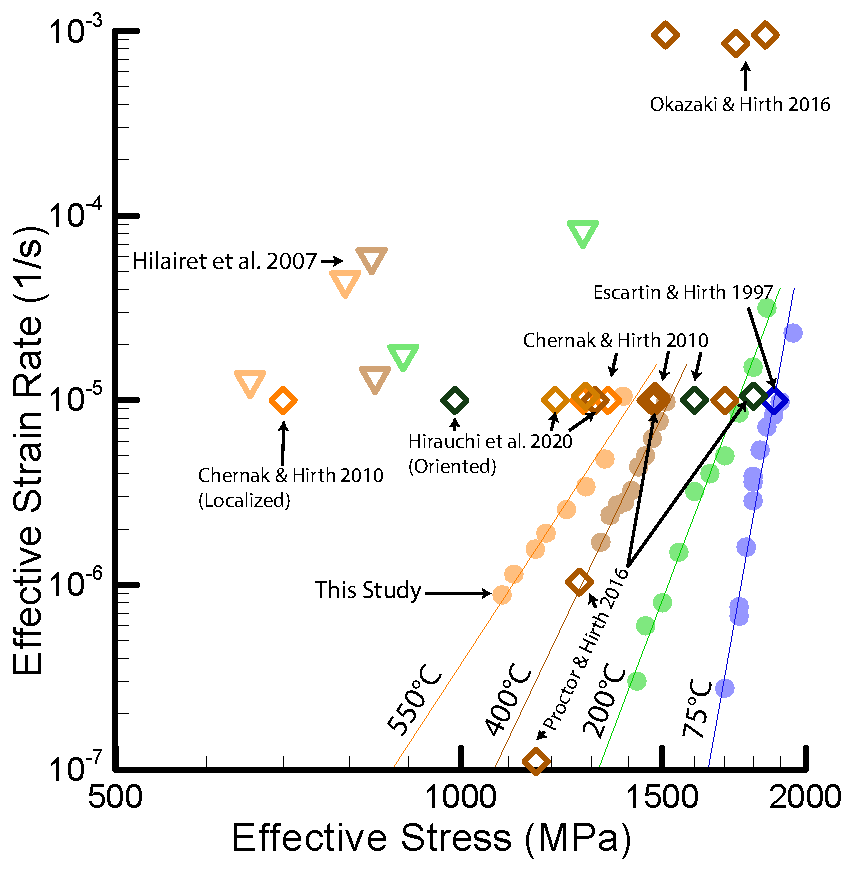
\includegraphics[width=\textwidth]{Figures/Creep Plot 9-20 comparison Annotatedv0.2.pdf}
  \caption[Compilation of our stress-strain rate points and other comparable tests]{
  Compilation of other high pressure experimental antigorite deformation results plotted over results form the current study. Colors of points denotes temperature for all points. Both cores \citep{hirauchi2020semi, Chernak2010, Escartin1997} and gouge \citep{Chernak2010, Proctor2016, Okazaki2016} are plotted.
  }
  \label{fig:CH2s_Data_Comparison_supplement}
\end{figure}

\begin{figure}
  \includegraphics[width=\textwidth]{Figures/Keishi_W15190914.jpg}
  \caption[Thin section image of SK-5 antigorite]{Thin section image (cross-polarized) of undeformed mesh texture. Compression of samples was in the vertical direction.
  }
  \label{fig:CH2s_ThinSection_Supplement}
\end{figure}

\begin{figure}
  \includegraphics[width=\textwidth]{Figures/All_cutopen.pdf}
  \caption[Macroscopic images of recovered antigorite creep specimens]{Images of antigorite core macrostructure. light/white portions of samples have shear microcracks.
  }
  \label{fig:CH2s_Macrostructure_Supplement}
\end{figure}

\begin{figure}
  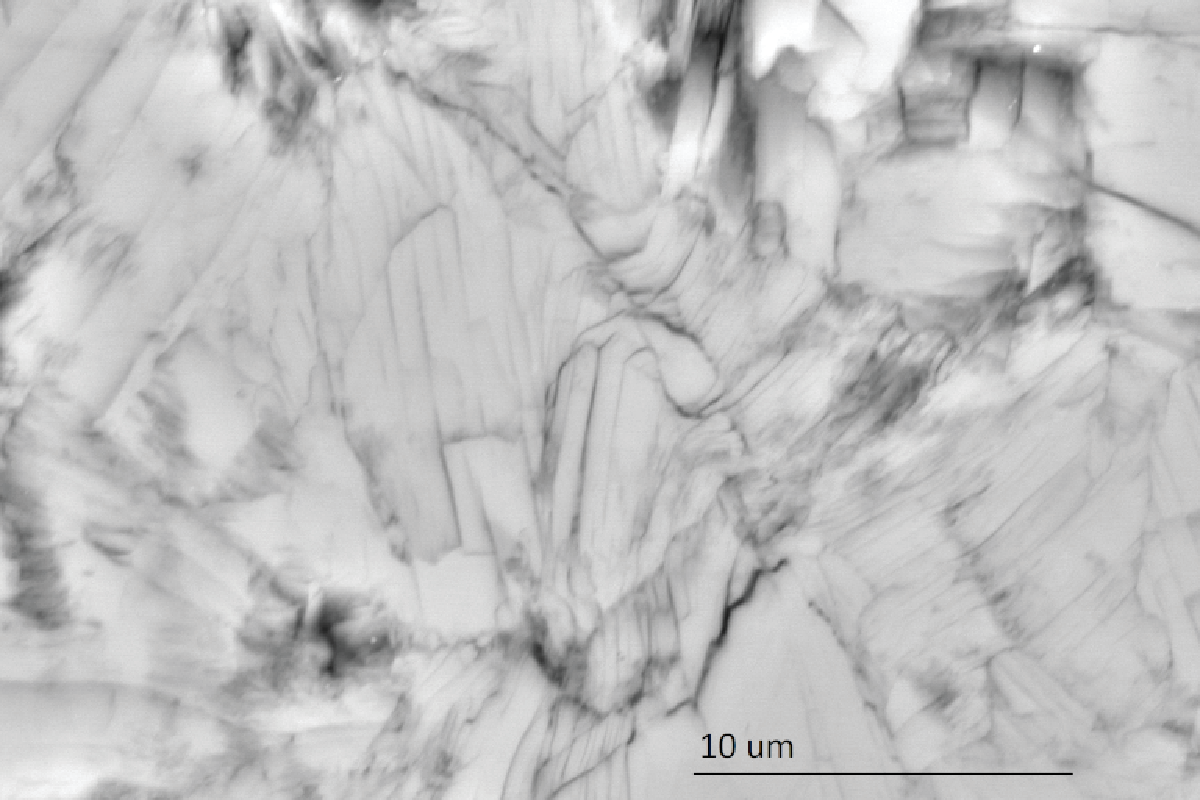
\includegraphics[width=\textwidth]{Figures/W2424_zoom005.pdf}
  \caption[SEM image of sheet curvature at 550C]{Gentle curvature of sheets recovered from 550°C sample.
  }
  \label{fig:CH2s_550C_Kinks_Supplement}
\end{figure}

\subsection{Hardening During Stress Steps} \label{CH2s_hardening_discussion}

    During individual stress steps samples harden over time (S\ref{fig:CH2s_Load-Time-Fast}). Hardening is expected to some extent from other descriptions/results of brittle creep and high temperature creep tests where primary, secondary, and tertiary creep phases can be identified. For westerly granite calibration tests (S\ref{fig:CH2s_Westerly_Supplement}), at each step samples reach constant strain rates after relatively small strains (~0.2\%). Post-processing of antigorite data shows that it may continue to harden over similar 0.2\% strain steps (depicted in data for W2447-200 (S\ref{fig:CH2s_Load-Time-Fast})). This decay is not obvious in live displays of data because it requires more processing power to smooth and compute than our rig control PC has available. 
    
    The observed rate decay appears to be linear when plotted as either log(strain rate) vs. strain (\ref{fig:CH2s_Strainrate-Strain}) and log(strain rate) vs. time (\ref{fig:CH2s_Strainrate-Time}). The strain rate decreases by approximately a factor of 2 over 0.2\% strain as can be observed in the included strain-time plots for W2447-200 (\ref{fig:CH2s_Load-Time-Fast}), and the decay during hydraulic oil confined experiment W2521-75 (\ref{fig:CH2s_Strainrate-Strain}). (Data is FIR decimated by a factor of 100 to 0.1Hz for these plots).

\begin{figure}
  \includegraphics[width=\textwidth]{Figures/W2447_StrainrateStrainStress.pdf}
  \caption[Experiment data from 200°C creep experiment]{Experiment data from 200°C experiment. black->stress; red->strainrate; cyan->strain (log scale).
  }
  \label{fig:CH2s_Load-Displacement}
\end{figure}

\begin{figure}
  \includegraphics[width=\textwidth]{Figures/W2447_1700MPa_LVDT2_trace_wlines.pdf}
  \caption[Load and displacement plotted against time to show strain rate evolution during a stress step]{Load and Displacement plotted against time to show strain rate evolution during a stress step. Data is taken from the last portion of the curve. Rate changes by approximately a factor of 2.
  }
  \label{fig:CH2s_Load-Time-Fast}
\end{figure}

\begin{figure}
  \includegraphics[width=\textwidth]{Figures/W2526_720MPa_LVDT2_trace_wlines.pdf}
  \caption[Load and Displacement plotted against time to show strain rate evolution during a low stress step]{Load and Displacement plotted against time to show strain rate evolution during a stress step. For "low" stresses, the displacement resolution limits determination of strain rate 
  }
  \label{fig:CH2s_Load-Time-Slow}
\end{figure}

%Greg thought these leave too much to interpretation
\begin{figure}
  \includegraphics[width=\textwidth]{Figures/W2521_stress_strainrate_vs_strain.pdf}
  \caption[Hardening of antigorite at room temperature vs. strain]{Hardening of antigorite at room temperature where rate change and stress are plotted against strain. Decay appears to be approximately log-linear.
  }
  \label{fig:CH2s_Strainrate-Strain}
\end{figure}

\begin{figure}
  \includegraphics[width=\textwidth]{Figures/W2521_stress_strainrate_vs_time.pdf}
  \caption[Hardening of antigorite at room temperature vs. stress]{Hardening of antigorite at room temperature where rate change and stress are plotted against time.
  }
  \label{fig:CH2s_Strainrate-Time}
\end{figure}



\subsection{Uncertainty introduced due to hardening} \label{CH2s_hardening_uncertainty}
    The ratio of initial/final strain seems to be similar at most stress steps. This makes ratio/increment (hardening slope) much larger at small strain. Hardening literature plots the change as $d\sigma/d\epsilon$ vs. $\sigma$ \citep{kocks2003physics}. It's unclear if that's appropriate for materials with pressure-dependent strength. 
    
    To assess the potential uncertainty introduced into the flow law by choosing final instead of initial strain rates, we re-plotted the fit for initial strain rates. Because change is a similar factor of ~2 for most steps, the fit exponent and athermal flow  stresses don’t change significantly while pre-exponential and activation energy change by ~5\%. % An example with the same exponents and peierls stress is plotted in Figure \ref{fig:CH2s_Hardening_Uncertainty}.

    In addition, our creep data can be compared to other antigorite deformation studies at similar temperatures and pressures \ref{fig:CH2s_Data_Comparison_supplement}. Some of the comparable studies use antigorite gouge instead of cores, which is noted. Despite widely varying methodology, recorded stress/strainrate is similar to other studies, except where samples are highly aligned or deformation is highly localized.

% \begin{figure}
%   \includegraphics[width=\textwidth]{Figures/Final-Initial Fit Comparison.png}
%   \caption[Comparison of hardening error in Peierls' fits]{Comparison of Peirels' fits of Final (Blue, lower), and initial (orange, higher) strain rates at each stress step.}
%   \label{fig:CH2s_Hardening_Uncertainty}
% \end{figure}

\subsection{Flow Law Fit Methodology} \label{CH2s_flowlawfit}
    A low temperature plasticity flow law was fit to stress vs. log(strainrate) using a Markov-chain Monte-Carlo (MCMC-NUTS) optimizer due to the small local discontinuities in the fit. Results with errors are presented in Table \ref{tab:CH2s_FitTable} and distributions of the posterior are plotted in figure S\ref{fig:CH2s_KDE_plot}.
    % \begin{table}[ht] % old!
    % \caption{Peierls creep fit results \label{tab:CH2s_FitTable}}
    % \begin{tabular}{lllll}
    % \hline
    %           & Mean   & Standard Deviation    & hdi\_2.5\% & hdi\_97.5\% \\
    % \hline
    % lnA  ln(1/s)        & -7.048  & 0.103 & 6.845      & 7.247       \\
    % Ea (kJ)         & 111.287 & 1.236  & 108.879     & 113.702      \\
    % Tau\_p (GPa)      & 2.537  & 0.032 & 2.477      & 2.601       \\
    % q          & 1.585  & 0.04  & 1.508      & 1.662       \\
    % $sigma_{obs}$ & 0.2    & 0.019 & 0.167      & 0.24       
    % \end{tabular}
    % \end{table}
    
    \begin{table}[ht]
    \caption{Low temperature plasticity creep fit results \label{tab:CH2s_FitTable}}
    \begin{tabular}{lllll}
    \hline
               & Mean   & Standard Deviation    & hdi\_2.5\% & hdi\_97.5\% \\
    \hline
    lnA ln(1/s) & -0.624 & 0.118 & -0.393 & -0.859 \\
    Ea (J) & 86283.744 & 1444.382 & 83395.443 & 89076.417 \\
    T\_p (GPa) & 2.416 & 0.044 & 2.330 & 2.502 \\
    q & 1.177 & 0.048 & 1.081 & 1.268 \\
    $sigma_{obs}$ & 0.215 & 0.020 & 0.176 & 0.255 \\  
    \end{tabular}
    \end{table}
    
    \begin{figure}
      \includegraphics[width=\textwidth]{Sections/Chapter2/Figures/MCMC_KDE_Matrix_StressSquared.png}
      \caption{Posterior probability density functions in parameter space for the MCMC fit.}
      \label{fig:CH2s_KDE_plot}
    \end{figure}
    
    Low stress data have a larger influence on the extrapolated fit because they define the transition between stress and temperature activation dominated regions of the Peierls law. The start of this transition can be seen in the slight curvature of the fit around points at 480°C in figure \ref{fig:CH2_Mechanical_combo}. In the flow law, the region is defined by exponents p, q, and normalization factor $\tau_p$.
    Changes in the curvature have a very large effect on extrapolated certainty of extrapolated viscosity. In this case feasible extrapolated viscosity decreases by several orders of magnitude when data at low stress is added to the fit (figure S\ref{fig:CH2s_Fitcompare-moredata}), and best fit confidence intervals shrink by an order of magnitude (figure \ref{fig:CH2_Mechanical_combo}).
    

\begin{figure}
  \includegraphics[width=\textwidth]{Sections/Chapter2/Figures/AtgVisc_StressSq_compare_1to1.pdf}
  \caption[Low temperature plasticity fit improvement with low strain rate data]{Comparison of fits for fixed exponent p,q combinations before and after slow strain  rate data is added to the dataset (for illustration). Slow strain rate data has a very strong effect on extrapolated viscosity.}
  \label{fig:CH2s_Fitcompare-moredata}
\end{figure}

\subsection{Griggs Rig Friction/Accuracy Measurement} \label{CH2s_frictiontesting}

    Several tests were completed to compare the new carbide bushing seal to the old mitre ring seal. We first deformed 360 grade brass rod, cut to simulate samples and confined by paraffin wax. The assembly was externally heated using hot water (same method as low temperature metal assembly), and repeatedly "hit" at different temperatures. (Figure \ref{fig:CH2s_Brass-Wax}) 
    We found that the squeezing force measured during “run-in”/"hit"  roughly follows predictions for “squeeze flow” rheometry. When the viscosity of the squeezed fluid decreases (in this case by heating the wax), the force for a given piston separation decreases.
    There is also a hysteresis with piston direction that does not vary significantly with temperature or distance between the sample and advancing piston. This appears to be primarily bearing friction applied by the packing ring. When we change to the carbide bushing, the size of the hysteresis loop decreases by a factor of 5x.
    Finally, rate dependence was explored with steps in the nearly fluid confining wax. Rate changes have a smaller effect with the carbide bushing (~2 MPa/10x strain rate), and do not have the small displacement dependent stress peaks the older mitre ring induces.
    
    To further test the ability to match the results of high temperature assemblies to room temperature assemblies, we loaded fused silica at 700°C in a standard, mitre-ring assembly and in a hydraulically confined assembly at low pressure (Figure \ref{fig:CH2s_WC-FS_elastic}). The results compare well, with the elastic modulus of the fused silica at high temperature matching the elastic modulus at low temperature. This indicates that we can compare all assemblies used in this study to each other and older results at similar conditions.

\begin{figure}
  \includegraphics[width=\textwidth]{Sections/Chapter2/Figures/Proposal_WaxCombo_small_clip.pdf}
  \caption[Friction testing of the modified carbide bushing in paraffin wax]{Plots of differential stress and displacement data from experiments deforming grade 360 (leaded) brass. Assemblies have no furnace, and all confining media is paraffin wax. Samples were first pressurized to 300 MPa. Then the piston was advanced towards the sample, retracted, heated, and advanced again repeatedly. Retraction is plotted as thin dotted lines. Hysteresis between advancing and advancing stresses is a measure of seal friction (30 MPa new carbide, 140 MPa old packing ring). Rate steps were completed while retracting far from the sample to measure rate dependent friction.
  }
  \label{fig:CH2s_Brass-Wax}
\end{figure}


\begin{figure}
  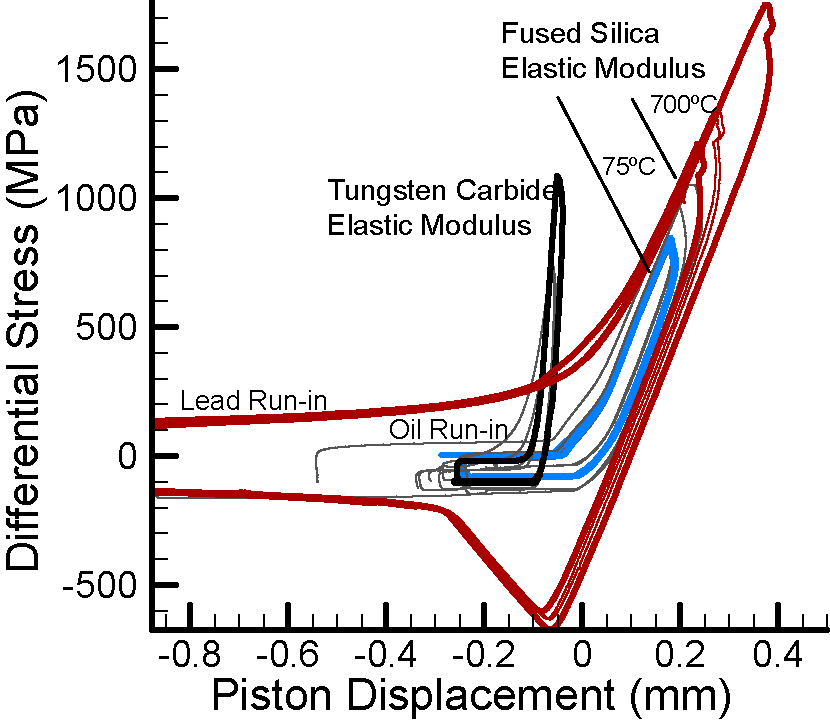
\includegraphics[width=\textwidth]{Figures/WC-FS_oil_HT.pdf}
  \caption[Elastic testing of fused silica at room temperature and 700°C]{Elastic tests of fused silica at room temperature in hydraulic oil and a solid salt assembly at 700°C with traditional packing rings. Despite the differences in friction and hit quality, load and displacement data match at high loads indicating correct calibration of our load and displacement transducers in both new and old assemblies.}
  \label{fig:CH2s_WC-FS_elastic}
\end{figure}

\begin{figure}
    \centering
    \includegraphics[width=\textwidth]{Sections/Chapter2/Figures/Thermal Model with TC_bp1 - Copy.pdf}
    \caption[Thermal model results]{Thermal model results. Methods are detailed in \citet{MOAREFVAND2021229032}}
    \label{fig:CH2s_ThermalModel}
\end{figure}


\begin{longtable}[c]{| m{0.65in} | m{0.65in} | c | c | c | c | c |}
    \caption[List of creep data used in Peierls' flow law]{Creep data \label{tab:CH2s_CreepFitPoints}}\\

    %\centering
    %\begin{tabular}{m{0.65in} m{0.65in} m{0.55in} m{0.55in} m{0.55in} m{0.45in} m{0.55in}}
    \hline
    Initial Strainrate (1/s) & Final Strainrate (1/s) & Initial Strain & Final Strain & Stress (MPa) & T (°C)    & Experiment \\
    \hline
    \endfirsthead
    
    \hline
    \multicolumn{7}{|c|}{Continuation of Table \ref{tab:CH2s_CreepFitPoints}}\\
    \hline
    \endhead
    
    \hline
    \endfoot
    
    \hline
    \multicolumn{7}{| c |}{End of Table}\\
    \hline\hline
    \endlastfoot
 
3.20E-06 & 2.85E-06 & 0.0001         & 0.0015       & 1800   & 75   & W2441      \\
7.80E-07 & 7.63E-07 & 0.0015         & 0.0022       & 1750   & 75   & W2441      \\
3.90E-06 & 3.87E-06 & 0.0022         & 0.0031       & 1800   & 75   & W2441      \\
7.53E-07 & 7.53E-07 & 0.0031         & 0.00345      & 1750   & 75   & W2441      \\
4.00E-07 & 2.75E-07 & 0.00345        & 0.0036       & 1700   & 75   & W2441      \\
9.00E-07 & 6.75E-07 & 0.0036         & 0.004        & 1750   & 75   & W2441      \\
4.00E-06 & 1.60E-06 & 0.004          & 0.0064       & 1775   & 75   & W2441      \\
6.80E-06 & 3.60E-06 & 0.0064         & 0.01         & 1800   & 75   & W2441      \\
9.40E-06           & 5.36E-06         & 0.01           & 0.016        & 1825   & 75   & W2441      \\
1.30E-05           & 7.15E-06         & 0.016          & 0.024        & 1850   & 75   & W2441      \\
1.42E-05           & 8.30E-06         & 0.024          & 0.034        & 1875   & 75   & W2441      \\
1.60E-05           & 9.80E-06         & 0.034          & 0.05         & 1900   & 75   & W2441      \\
3.00E-05           & 2.31E-05         & 0.05           & 0.07         & 1950   & 75   & W2441      \\
8.00E-07           & 3.00E-07         & 0.00042        & 0.00087      & 1425   & 200  & W2447      \\
1.00E-06           & 6.00E-07         & 0.00087        & 0.0011       & 1450   & 200  & W2447      \\
1.00E-06           & 8.00E-07         & 0.0011         & 0.00178      & 1500   & 200  & W2447      \\
2.20E-06           & 1.50E-06         & 0.00178        & 0.00268      & 1550   & 200  & W2447      \\
5.00E-06           & 3.20E-06         & 0.00268        & 0.00338      & 1600   & 200  & W2447      \\
7.00E-06           & 4.00E-06         & 0.00338        & 0.00423      & 1650   & 200  & W2447      \\
1.10E-05           & 5.00E-06         & 0.00423        & 0.00559      & 1700   & 200  & W2447      \\
1.30E-05           & 8.51E-06         & 0.00559        & 0.0071       & 1750   & 200  & W2447      \\
2.60E-05           & 1.51E-05         & 0.0071         & 0.0096       & 1800   & 200  & W2447      \\
5.20E-05           & 3.16E-05         & 0.0096         & 0.0148       & 1850   & 200  & W2447      \\
2.25E-06           & 1.70E-06         & 0.0055         & 0.007        & 1325   & 400  & W2439      \\
2.80E-06           & 2.38E-06         & 0.007          & 0.009        & 1350   & 400  & W2439      \\
3.40E-06           & 2.70E-06         & 0.009          & 0.011        & 1370   & 400  & W2439      \\
3.80E-06           & 2.80E-06         & 0.011          & 0.0133       & 1390   & 400  & W2439      \\
4.00E-06           & 3.24E-06         & 0.0133         & 0.016        & 1410   & 400  & W2439      \\
5.00E-06           & 4.35E-06         & 0.016          & 0.019        & 1430   & 400  & W2439      \\
6.90E-06           & 5.00E-06         & 0.019          & 0.023        & 1450   & 400  & W2439      \\
7.80E-06           & 6.20E-06         & 0.023          & 0.028        & 1470   & 400  & W2439      \\
9.40E-06           & 7.70E-06         & 0.028          & 0.0325       & 1490   & 400  & W2439      \\
1.05E-05           & 9.80E-06         & 0.0325         & 0.036        & 1510   & 400  & W2439      \\
1.40E-06           & 8.82E-07         & 0.0005         & 0.00138      & 1062   & 550  & W2424      \\
1.60E-06           & 1.14E-06         & 0.00138        & 0.0024       & 1088   & 550  & W2424      \\
3.00E-06           & 1.56E-06         & 0.0024         & 0.00373      & 1137   & 550  & W2424      \\
2.60E-06           & 1.90E-06         & 0.00373        & 0.00474      & 1162   & 550  & W2424      \\
5.40E-06           & 2.56E-06         & 0.00474        & 0.00705      & 1212   & 550  & W2424      \\
7.50E-06           & 3.40E-06         & 0.00705        & 0.0106       & 1261   & 550  & W2424      \\
9.00E-06           & 4.80E-06         & 0.0106         & 0.015        & 1311   & 550  & W2424      \\
1.40E-05           & 1.05E-05         & 0.015          & 0.023        & 1361   & 550  & W2424      \\
8.00E-09           & 5.00E-09         & 0.0001         & 0.001        & 480    & 520  & W2520      \\
2.20E-08           & 1.70E-08         & 0.001          & 0.0022       & 600    & 520  & W2520      \\
4.00E-08           & 3.40E-08         & 0.0022         & 0.0033       & 690    & 520  & W2520      \\
8.00E-08           & 6.00E-08         & 0.0033         & 0.0048       & 790    & 520  & W2520      \\
9.50E-08           & 7.50E-08         & 0.0048         & 0.0063       & 880    & 520  & W2520      \\
5.00E-09           & 4.50E-09         & 0.0063         & 0.0067       & 470    & 520  & W2520      \\
1.40E-07           & 1.20E-07         & 0.0067         & 0.018        & 970    & 520  & W2520      \\
1.41E-09           & 1.40E-09         & 0.0001         & 0.0003       & 1230   & 76   & W2521      \\
4.00E-09           & 2.50E-09         & 0.0003         & 0.0005       & 1280   & 76   & W2521      \\
8.00E-08           & 5.00E-09         & 0.0005         & 0.0008       & 1330   & 76   & W2521      \\
2.50E-08           & 1.50E-08         & 0.0008         & 0.0015       & 1380   & 76   & W2521      \\
5.00E-08           & 3.00E-08         & 0.0015         & 0.0028       & 1430   & 76   & W2521      \\
2.50E-07           & 6.00E-08         & 0.0028         & 0.0046       & 1480   & 76   & W2521      \\
1.60E-06           & 1.50E-07         & 0.0046         & 0.00758      & 1550   & 76   & W2521      \\
1.50E-06           & 3.00E-07         & 0.00758        & 0.011        & 1580   & 76   & W2521      \\
2.00E-06           & 6.00E-07         & 0.011          & 0.0147       & 1600   & 76   & W2521      \\
2.20E-06           & 5.00E-07         & 0.0147         & 0.0198       & 1650   & 76   & W2521      \\
3.30E-06           & 1.00E-06         & 0.0198         & 0.022        & 1700   & 76   & W2521      \\
9.00E-06           & 2.00E-06         & 0.022          & 0.0257       & 1750   & 76   & W2521      \\
1.20E-05           & 5.00E-06         & 0.0257         & 0.032        & 1800   & 76   & W2521      \\
1.10E-08           & 3.00E-09         & 0.0323         & 0.0325       & 1510   & 76   & W2521      \\
8.00E-09           & 6.00E-09         & 0.0325         & 0.0326       & 1560   & 76   & W2521      \\
1.10E-08           & 8.00E-09         & 0.0326         & 0.0328       & 1620   & 76   & W2521      \\
1.50E-08           & 8.00E-09         & 0.0328         & 0.033        & 1670   & 76   & W2521      \\
2.30E-08           & 2.00E-08         & 0.033          & 0.0333       & 1710   & 76   & W2521      \\
1.00E-07           & 4.00E-08         & 0.0333         & 0.0353       & 1720   & 76   & W2521      \\
3.20E-07           & 1.50E-07         & 0.0353         & 0.0383       & 1750   & 76   & W2521      \\
7.00E-08           & 1.50E-08         & 0.0001         & 0.0002       & 635    & 480  & W2526      \\
5.00E-09           & 2.50E-09         & 0.0002         & 0.0005       & 475    & 480  & W2526      \\
1.00E-08           & 7.50E-09         & 0.0005         & 0.001        & 575    & 480  & W2526      \\
1.20E-08           & 1.00E-08         & 0.001          & 0.0013       & 645    & 480  & W2526      \\
3.00E-08           & 2.50E-08         & 0.0013         & 0.0021       & 725    & 480  & W2526      \\
2.00E-07           & 1.50E-07         & 0.0021         & 0.0028       & 975    & 480  & W2526      \\
8.00E-09           & 5.00E-09         & 0.0028         & 0.0032       & 505    & 480  & W2526      \\
1.50E-08           & 9.00E-09         & 0.0032         & 0.0036       & 595    & 480  & W2526      \\
1.90E-08           & 1.50E-08         & 0.0036         & 0.004        & 695    & 480  & W2526      \\
3.50E-08           & 3.00E-08         & 0.004          & 0.0044       & 795    & 480  & W2526      \\
%\end{tabular}
\end{longtable} 


\end{document}